\documentclass[5p,authoryear]{elsarticle}
\makeatletter 
\def\ps@pprintTitle{%
 \let\@oddhead\@empty
 \let\@evenhead\@empty
 \let\@evenfoot\@oddfoot} % Supprimer le bas de page ELSEVIER
\makeatother
\usepackage[utf8]{inputenc} % En unicode
\usepackage[T1]{fontenc}
\usepackage[english]{babel}
\usepackage[babel=true]{csquotes} % permet de faire \enquote{a} (« a »)
\usepackage[fleqn]{amsmath} % pour certains signes mathématiques
\usepackage{amsthm} % Pour \begin{gather}
\usepackage{booktabs} % pour \toprule (un style de tableau)
\usepackage{multirow} % Pour colonnes multiples des tableaux
\usepackage{amssymb} % Pour \leqslant (<=, >=)
\usepackage{float}
\usepackage{hyperref} % 
\usepackage[english]{cleveref} 




%\bibliographystyle{elsarticle-num}
\bibliographystyle{elsarticle-harv}

\usepackage{fancyhdr}
\pagestyle{fancy}
\lhead{MSDS 458 - SEC 56}
\rhead{Lee, J.}

\begin{document}

\begin{frontmatter}

\title{Gambling Twitter Bot: Natural Language Processing –\\ A Recurrent Neural Network Analysis}
% Research Assignment 2
%% Group authors per affiliation:
\author{Jason Lee}
\address{Northwestern University, SPS \\Artificial Intelligence and Deep Learning \\2019FA MSDS 458-56}


\begin{abstract}

Artificial neural networks are extremely powerful algorithms that are able to solve very complicated problems. This paper investigates the difference in performance between fully connected artificial neural networks (DNNs), one-dimensional convolutional neural networks (CNNs), and recurrent neural networks (RNNs) with regard to natural language processing (NLP) tasks. It is important to understand when and how to utilize the various types of networks available when building deep (multiple hidden layers) neural networks to solve language problems. The goal of this study centers around the predictive performance classifying Twitter users by their tweets.



\end{abstract}


\begin{keyword}
Recurrent Neural Networks \sep Deep Learning \sep Natural Language Processing (NLP) \sep Keras\end{keyword}

\end{frontmatter}



%\linenumbers
\section{Introduction}\label{introduction}

Understanding all the nuances of language is a complex task for humans and computers alike. The intricacies of language and syntax have created dedicated fields of study for researchers. There are numerous synonyms, homonyms, and antonyms for people to use. A sequence of words or groupings of words can change the entire meaning in a sentence. These examples make it increasingly difficult for a computer to interpret meaning. For example, the word “Lead” can be used in several different ways. 

It could be used as a noun meaning someone is in first place: 

\begin{displayquote}
“The Kansas City Chiefs are in the lead!”
\end{displayquote}


It could be a verb where someone is guiding someone else:

\begin{displayquote}
“The Chiefs lead the movement of high-power passing offenses in the NFL.”
\end{displayquote}


Or the exact same spelling is a completely different word meaning a type of metal with a different pronunciation: 

\begin{displayquote}
“The Chiefs’ stadium has lead under each chair.”
\end{displayquote}


These four letters grouped together making the word “Lead” provide a different meaning in each of these sentences. This is just one of many examples where word usage causes problems for machine learning. However, many complex natural language problems can be solved by using a special type of deep learning model called a recurrent neural network (RNN). 

Chatbots, predictive texting, language translation, sentiment analysis of business reviews, determining an author based on their previous work, identifying an article’s topic, automated summarizing of news articles, and automatic captioning of images and videos are all real-world applications of recurrent neural network models. These models can help improve efficiency in business operations and in daily life.

For natural language processing (NLP) tasks, using a dense, or fully connected, neural network is similar to breaking a sentence into individual words, mixing them up, and then trying to decipher what the mess of random words actually mean. Unfortunately for these dense neural networks, the location and context of words are what give the sentence meaning. This is where recurrent neural networks shine.

Recurrent neural networks are fed sequential data, like a string of words creating a sentence. The RNN is able to remember what words have come before because the output from each step (word) in the model is fed back into the model as an input for the next step (word). These models are able to extract meaningful patterns in the words the same way convolutional neural networks are able to recognize important patterns in the pixels for computer vision. 

This study will focus on a natural language problem classifying Twitter users based on their tweets. Individuals use language in subtly unique ways that may go unnoticed by human observers. These differences can be detected by an algorithm that can use these differences to identify a specific user from other users. 

The purpose of this analysis is three-fold: 1 – Determine the proper way to construct a trustworthy deep neural network for natural language processing tasks. 2 – Evaluate the training time and overall prediction accuracy between the various neural network architectures. 3 – Generate a reproducible Python workflow with a working prediction model to easily share with colleagues. 



\subsection{Twitter Users’ Tweets – Sports Betting Community} \label{twitter}

To accomplish the goal of this study, 42 popular twitter users in the sports betting community were selected. The classification problem will be to determine which twitter user wrote which tweets. The data feeding the models will exclude any retweets from the user, focusing solely on the original author’s tweets to analyze linguistic tone, style, content, and sentiment. This particular task will be difficult as there are many users in this space who sound very similar and many tweets only contain a handful of words. However, these models will also be able to give a glimpse into which users are more closely related.

Figures \ref{aisports}, \ref{rufus}, \ref{cousin}, and \ref{joey} provide samples of tweets from various Twitter users. The topics, lengths, and spelling can vary dramatically from tweet to tweet and from user to user making the learning task much harder for an algorithm with no domain knowledge.


\begin{figure}[!htb] \centering
	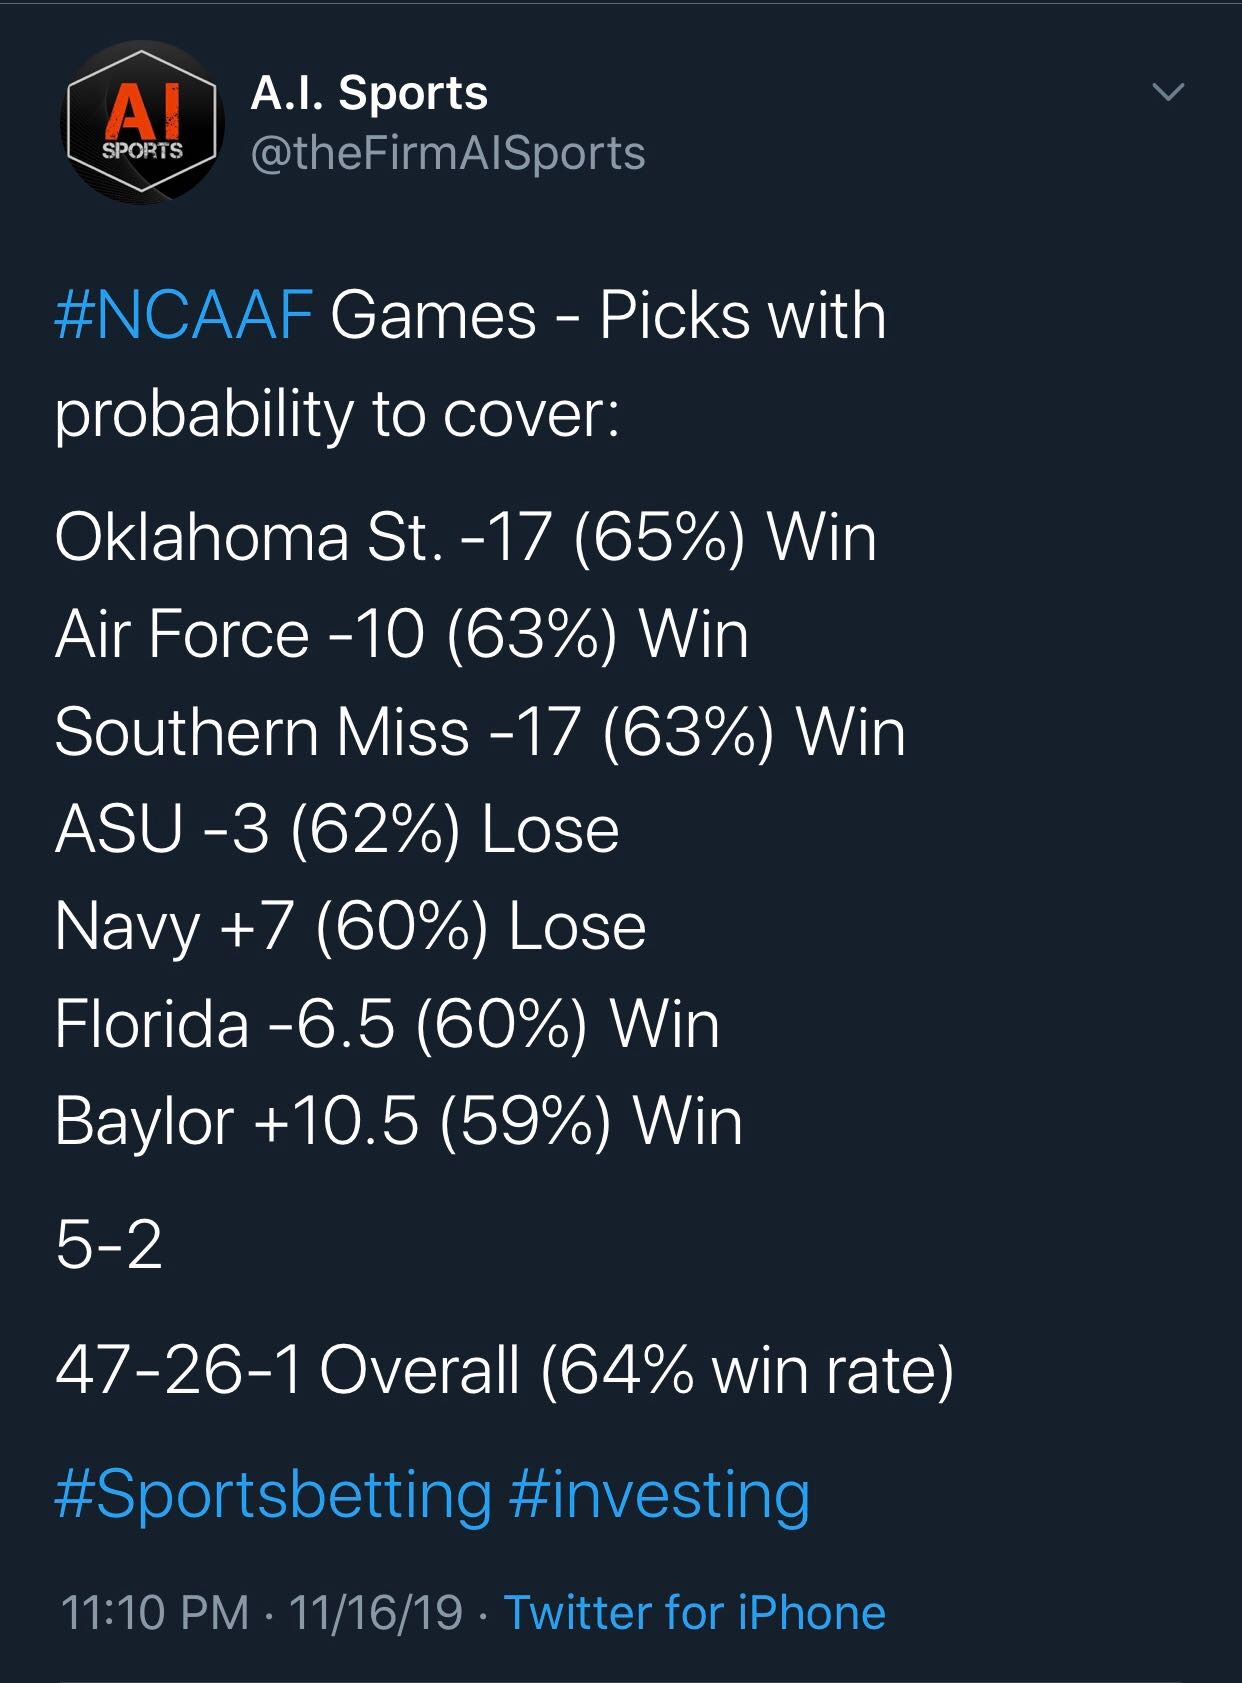
\includegraphics[width=3.4in]{figures/AISports_Tweet.jpg}
	\caption[]{Random sample tweet from A.I. Sports showing their particular style and tone} \label{aisports} 
\end{figure}


\begin{figure}[!htb] \centering
	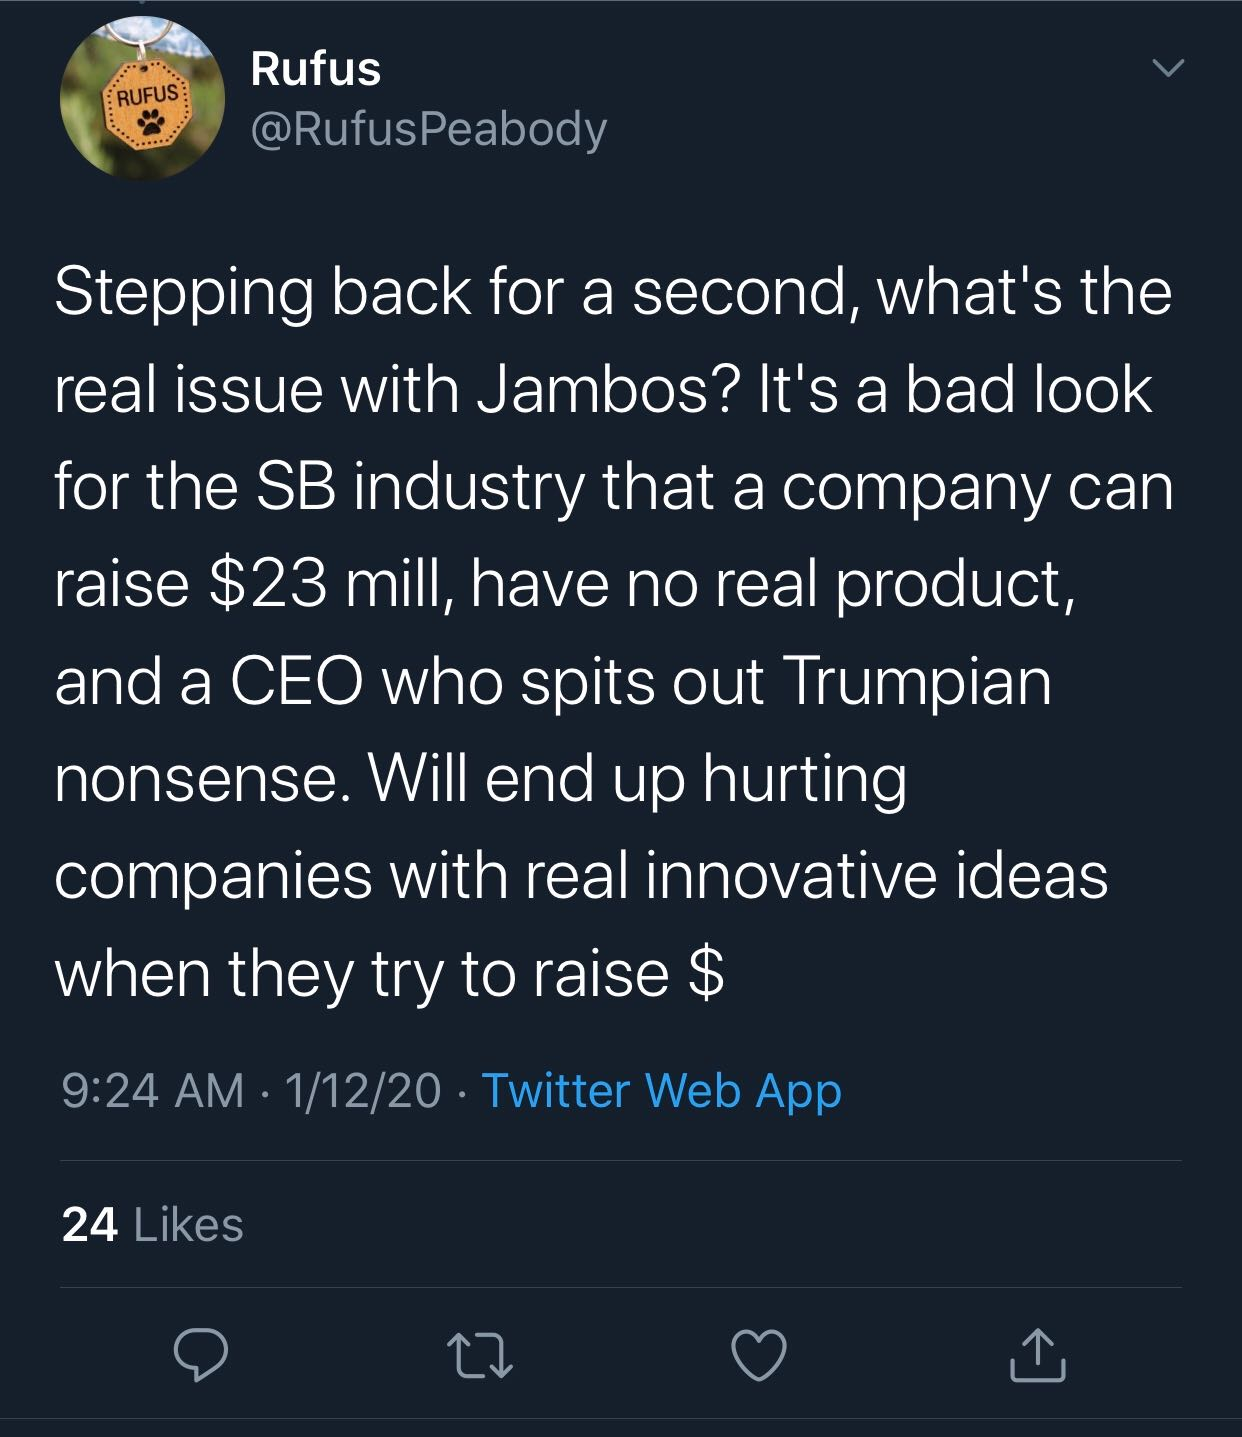
\includegraphics[width=3.4in]{figures/Rufus_Tweet.jpg}
	\caption[]{Random sample tweet from Rufus Peabody showing his particular style and tone} 
	\label{rufus} 
\end{figure}


\begin{figure}[!htb] \centering
	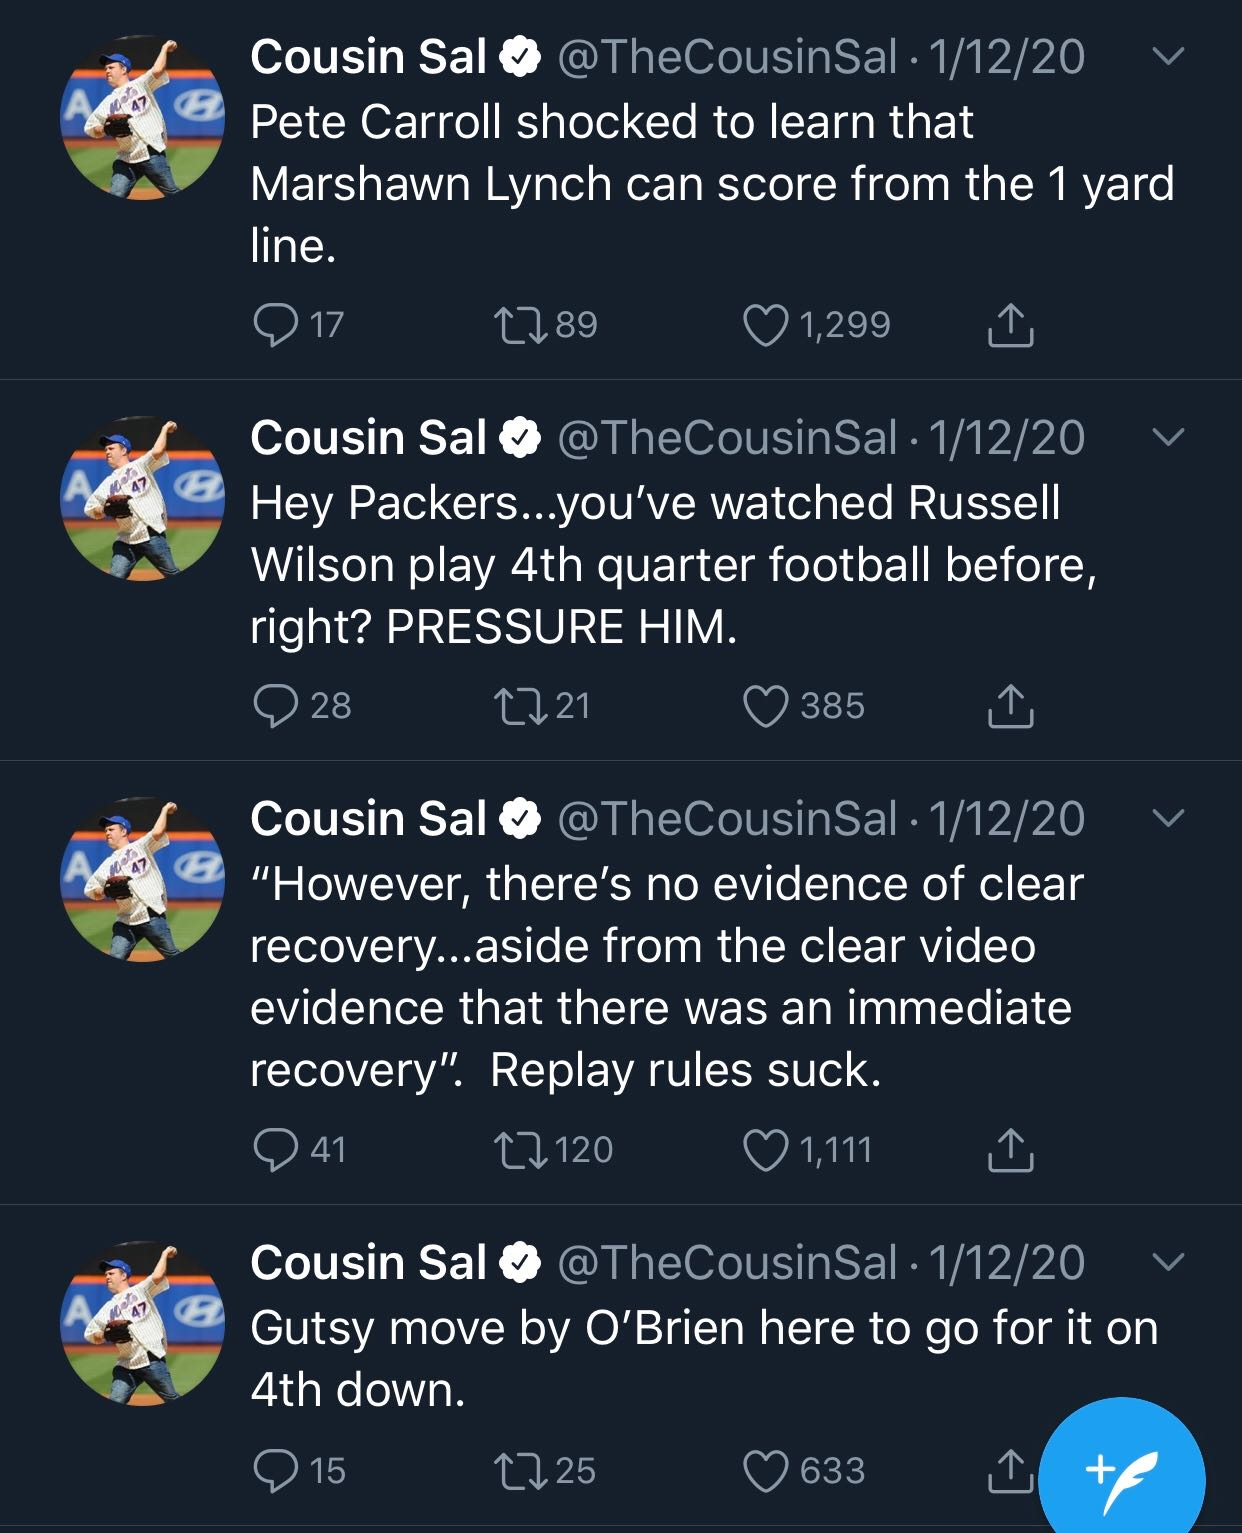
\includegraphics[width=3.4in]{figures/CousinSal_Tweet.jpg}
	\caption[]{4 Sample tweets from Cousin Sal showing his style and tone} 
	\label{cousin} 
\end{figure}



\begin{figure}[!htb] \centering
	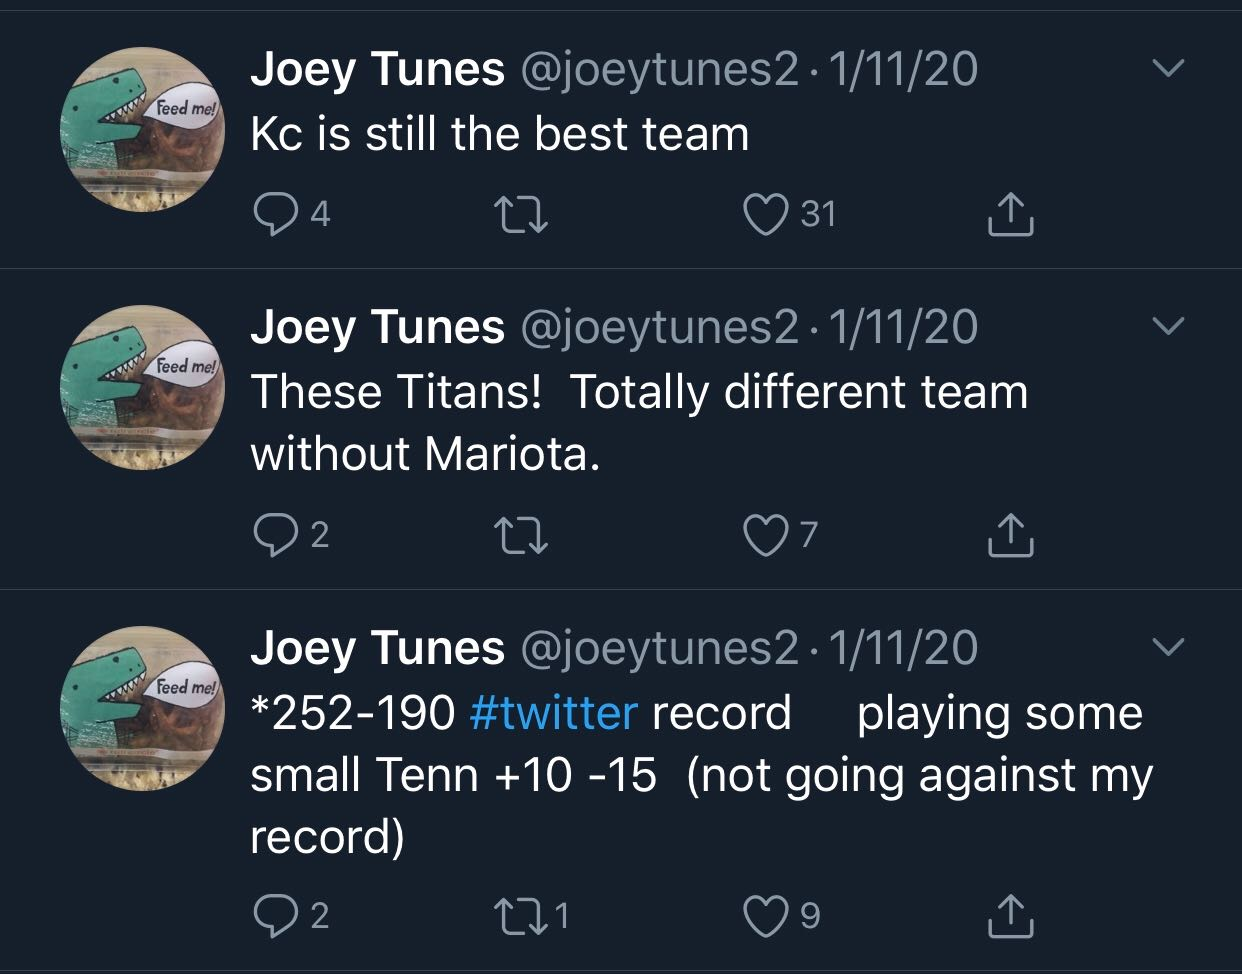
\includegraphics[width=3.4in]{figures/JoeyTunes_Tweet.jpg}
	\caption[]{3 Sample tweets from Joey Tunes showing his style and tone} 
	\label{joey} 
\end{figure}



\section{Literature Review} \label{lit_rev}

When it comes to language, the order of words impacts the meaning of the sentence. The benefit of using recurrent neural networks over a standard dense neural network is that the RNNs are able to interpret language with context and order intact. They consume sentences word by word learning more as the sequence of words grows.


\begin{figure}[!h] 
    \centering
	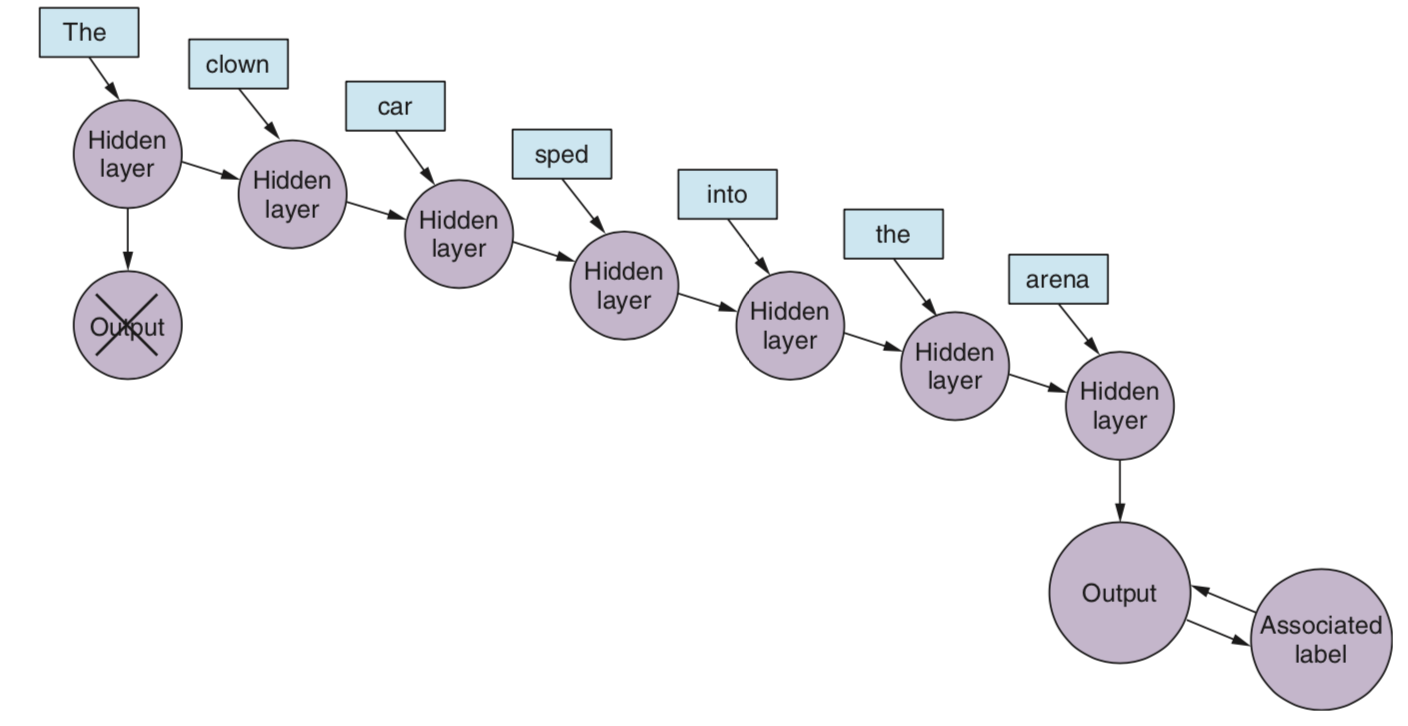
\includegraphics[width=3.4in]{figures/RNN_Flow.png}
	\caption[]{Recurrent Neural Network Model Flow} 
	\label{RNN_flow} 
\end{figure}

Figure \ref{RNN_flow} visualizes a simple recurrent neural network model flow when given the sentence “The clown car sped into the arena.” The model receives the first word “The” and creates an output. That output is hidden and carried over as an input into the model with the second word “clown”. At the third step, the model has the output from “The clown” and adds “car”. By the time we get to the end of the sentence, the recurrent neural network is able to process the entire sentence in the same order that a human would read it. This will allow the model to understand the high-level meaning of the sentence and learn the context of each word in the sentence \citep{chollet}. After the entire sentence is processed, the model is able to produce a label, sentiment, translation, response, etc. 

Similar to basic neural networks, a recurrent neural network is a mathematically dependent model that receives input data and produces an output based on strict mathematical rules. These models are able to improve, or learn, over the course of their training time as internal weights are updated along a gradient in a feedback loop \citep{lane}. The performance of any deep learning model is dependent on how each layer is stacked, how the hyperparameters are tuned, and what training, validation, and testing datasets are used. 

One-dimensional convolutional neural networks are also able to properly order words in a sentence. Convolutional neural networks excel with computer vision by using small window inputs that slide across the images searching for specific patterns as was shown in the last study \citep{lee}. One-dimensional convolutional neural networks use a window that moves from left to right across a sentence taking in small groups of words at a time extracting meaningful patterns \citep{chollet}. Figure \ref{CNN_flow} visualizes the window movement of the CNN across two different sentences. The model takes in two words at a time and slides to the right by one word to create a new input for the model.

\begin{figure}[!h] 
    \centering
	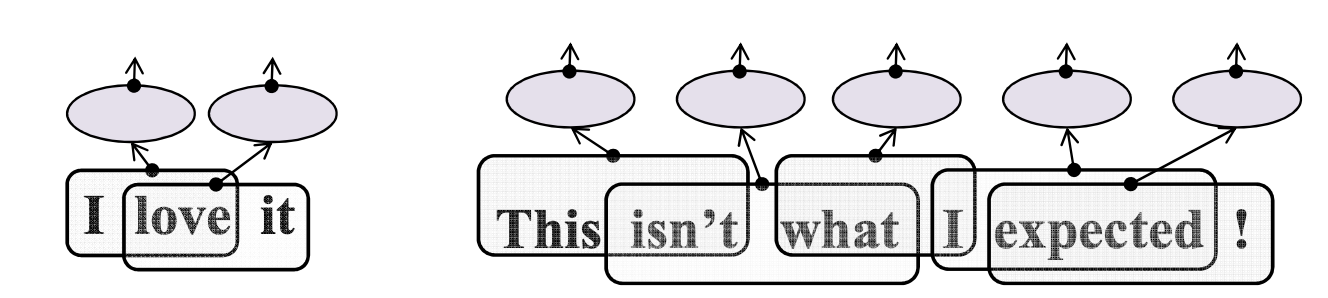
\includegraphics[width=3.4in]{figures/1D_CNN.png}
	\caption[]{One-Dimensional Convolutional Neural Network Model window flow over text} 
	\label{CNN_flow} 
\end{figure}



\subsection{Text Tokenization and Encoding}\label{token}

In order to develop a natural language processing algorithm, each sentence needs to be broken down into individual units. This process is known as text tokenization. The specific unit size can vary. Depending on the model, the token may either represent a single character, a single word, group of words, or n-grams \citep{chollet}. N-gram tokens are overlapping sequenced groups of words or characters.

To illustrate text tokenization, Figure \ref{tokenpic} provides a simple sentence about the sports betting contest landscape in America. This sentence will be transformed into tokens by word. This single sentence now becomes nine tokens.


\begin{figure}[!h] 
    \centering
	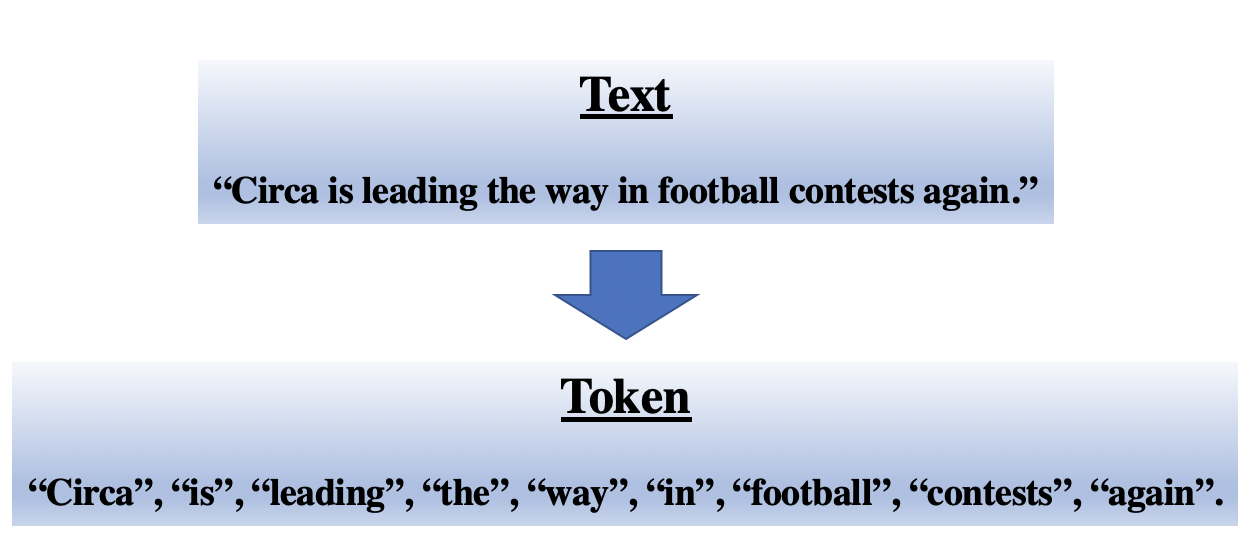
\includegraphics[width=3.4in]{figures/Text_Tokenization.png}
	\caption[]{Example converting a sentence into tokens} 
	\label{tokenpic} 
\end{figure}

However, the model will not be able to interpret these newly created tokens yet either. The algorithm can only be fed numeric values in order for it to perform the mathematical calculations. The next step is to convert each token into a numeric vector. One hot encoding is a very common process where each unique token is given a unique index in the vector space where the token will have a binary flag in its index and zeros everywhere else \citep{mool}. There are around 20,000 common words and into the millions when including proper nouns and names \citep{lane}. One hot encoding could easily result in a vector with over 100,000 dimensions. The issue with one hot encoding the tokens is that it will create a high dimensional, sparse dataset that will be computationally expensive for the model to train \citep{chollet}. 

Another method to transform tokens into numbers is by using vector encodings, also known as embeddings. They are able to compress all of the tokens into a dense vector with a specified output dimension. Figure \ref{encoded} shows how the example sentence tokens are encoded into a numeric vector of three dimensions; each word has been boiled down to only three numbers.


\begin{figure}[!h] 
    \centering
	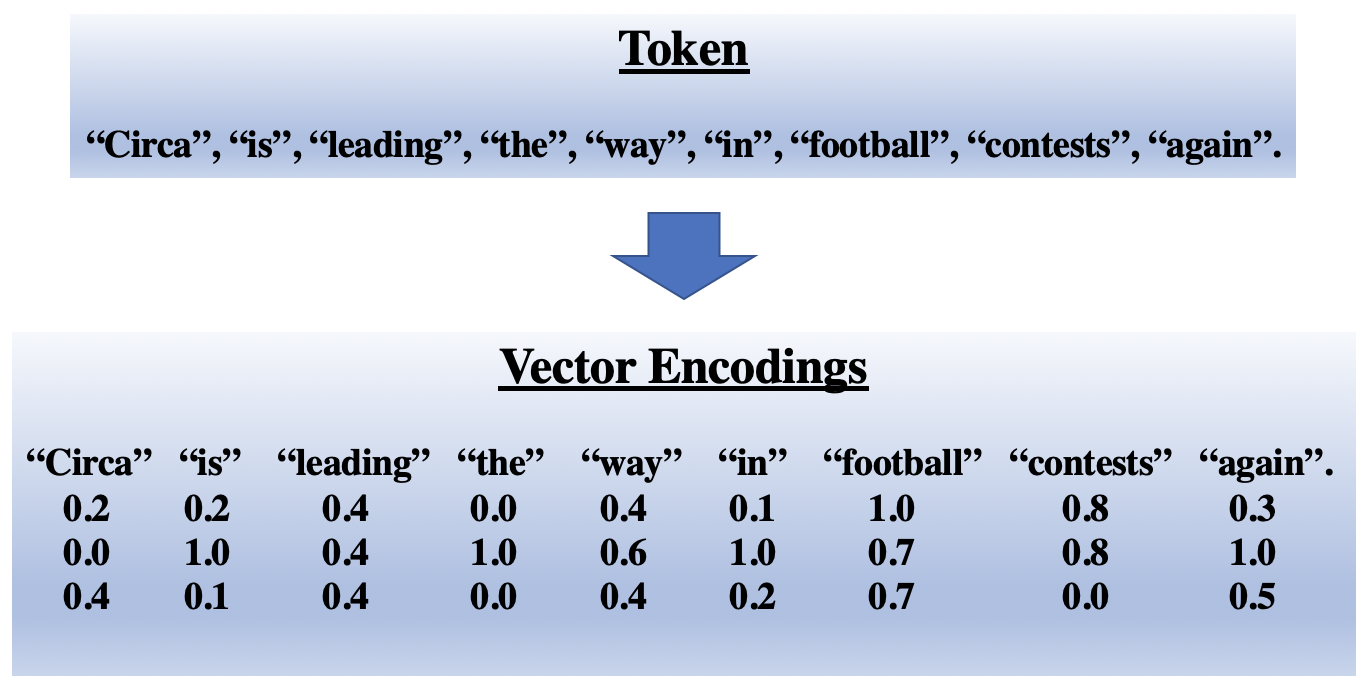
\includegraphics[width=3.4in]{figures/Vector_Encoding.png}
	\caption[]{Example generating vector encodings from word tokens} 
	\label{encoded} 
\end{figure}



\subsection{Trained Word Embeddings}\label{embedding}

Vectorizing words on its own does not add any context or meaning. This is where a properly trained word embedding layer comes into play. Conceptually, the embedding layer places word vectors into a geometric space where the Euclidean distance between words creates context and meaning \citep{chollet}. The distance in this new geometric space parallels the distance between the words’ semantic meaning. For example, the mathematical result when subtracting each one of these pairs are nearly equivalent when using a pre-trained word embedding layer.


Properly trained word embeddings allow one to perform mathematical computations with words to better understand language. For example, the embedding vector representing “King” subtracted by the embedding vector representing “Male” will equivalent to the embedding vector representing “Queen.”

$$King-Male=Queen$$

This is a simple equation for humans to solve but understanding the words’ relationship in this way for computers was a groundbreaking advancement. 

There are two main open sourced pre-trained word embedding models: The Word2Vec model created by Thomas Mikolov at Google and the GloVe model out of Stanford created by Jeffrey Pennington, Richard Socher, and Christopher Manning. The methodologies to create the embeddings are very different with the GloVe model using a global word-to-word co-occurrence metric trained on wikipedia pages covering 6 billion tokens and a vocabulary size of 400,000 \citep{glove} and the Word2Vec model using a two-layer neural network trained on 100 billion words from the Google News Corpus with a vocabulary size of 3 million \citep{word2vec}. While their methodologies differ, both embedding models reach very similar conclusions when performing the equations above. These models also allow computers to solve analogies, retrieve most similar words, query text, and calculate the distance between words.



\subsection{Long Short-Term Memory (LSTM)}\label{LSTM}

In practice, recurrent neural networks struggle to train properly because of an issue discovered by Hochreiter and Schmidhuber called the vanishing gradient (Hochreiter & Schmidhuber, 1997). As recurrent neural networks learn from the data during each epoch, the model may “get stuck” when the updated error value passed back through the network becomes so miniscule that there are effectually no changes made to the internal weights. Another issue recurrent neural networks run into because of the looping from output to input is the fact that they are extremely computationally expensive and inefficient to train. Hochreiter and Schmidhuber were able to address both of these issues by creating a Long Short-Term Memory cell (LSTM). The long short-term memory cell stores unchanged information from previous time steps allowing the model to access that data when needed. This method has enhanced training times and performance of recurrent neural networks, and even solving previously unsolvable complex problems by other recurrent neural networks (Hochreiter & Schmidhuber, 1997).




\subsection{Bidirectional RNN}\label{BiRNN}


Another tool developed to increase the predictive power when modeling sequential data like natural language processing tasks is a bidirectional recurrent neural network (Bi-RNN). Human brains are able to move back to earlier parts of a sentence when new information is presented seamlessly to process the entire sentence’s meaning. A bidirectional recurrent neural network is able to read the sentence forward and backwards extracting new relationships and meaning that help improve the model’s performance \citep{lane}. Figure \ref{BiRNN_Flow} shows the parallel nature of a Bi-RNN. Two models are created with different inputs and are combined together to produce an output.


\begin{figure}[!h] 
    \centering
	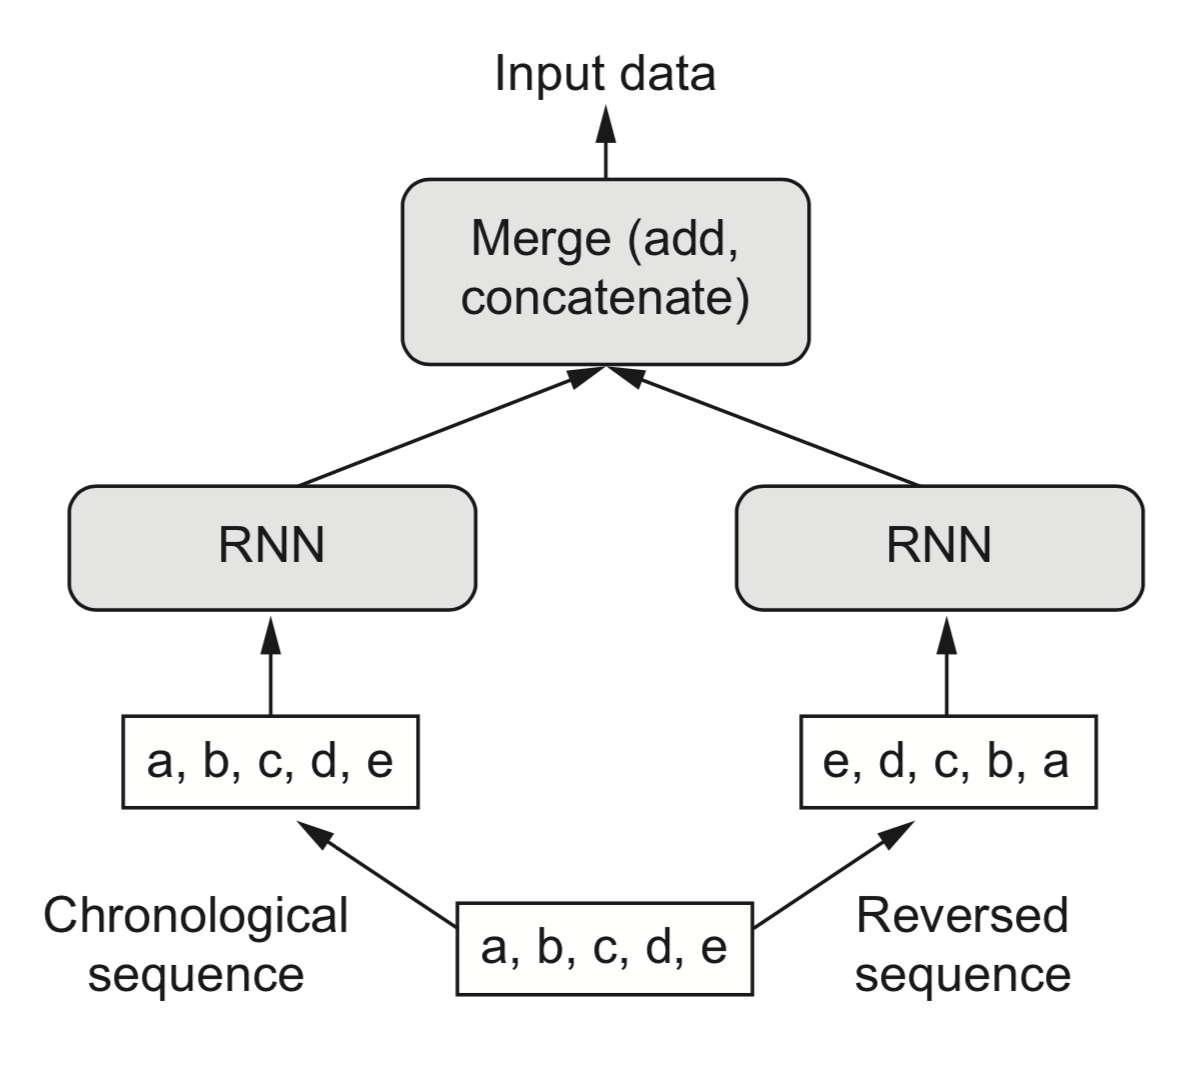
\includegraphics[width=3.4in]{figures/Bi-RNN_Flow.png}
	\caption[]{Bidirectional Recurrent Network Flow} 
	\label{BiRNN_Flow} 
\end{figure}


\section{Methodology}\label{meth}

The methodology undertaken in this study is as follows. There will be four distinct neural networks trained to classify gambling twitter users based on their tweets. The Keras package in Python, which is built on TensorFlow, will be used to develop each of the four deep neural networks. Each model will use the same training, validation, and testing datasets to provide a consistent comparison of model accuracy and training times. The mini batch size for each model’s training will be fixed at 32 and the training will run for a total duration of 10 epochs. The optimization function used for all models will be the Adaptive Moment Estimation (Adam) optimizer in the Keras package. The models will all conclude with a densely connected output layer using the softmax activation function for the 42 predictive classes of gambling twitter users.



\subsection{Neural Network Architecture}\label{arch}

There will be four unique deep neural network architectures built in this study. The first neural network will be a fully connected, or dense, neural network (DNN). The second neural network will be a one-dimensional convolutional neural network (CNN). The third neural network will be recurrent neural network (RNN) with long short-term memory (LSTM). The final neural network will utilize a bidirectional LSTM recurrent neural network structure (Bi-RNN).

\subsubsection{Dense Neural Network (DNN)}\label{dnn}

The DNN Model will have 6 steps with 14,162,794 total parameters, of which 962,794 are trainable.

\begin{enumerate}
 \item Input Layer – (Sequence of 50 Words)
 \item Embedding – (13,200,000 fixed parameters)
 \item Flatten
 \item Dense Layer - (960,064 parameters)
 \item Dropout - 30\%
 \item Dense Output Layer - (2,730 parameters)
\end{enumerate} \\

\subsubsection{1D Convolutional Neural Network (CNN)}\label{cnn}

1D-CNN will have 8 steps in its model with 13,623,542 total parameters, of which only 423,542 parameters are trainable.

\begin{enumerate}
 \item Input Layer – (Sequence of 50 Words)
 \item Embedding – (13,200,000 fixed parameters)
 \item Convolutional Layer – (225,250 parameters)
 \item Dropout - 30\%
 \item Convolutional Layer – (187,750 parameters)
 \item Dropout - 30\%
 \item Pooling Layer
 \item Dense Output Layer - (10,542 parameters)
\end{enumerate} \\


\subsubsection{LSTM Recurrent Neural Network (RNN)}\label{rnn}

The RNN model will have 6 steps with 13,650,842 total parameters, of which only 450,842 are trainable.

\begin{enumerate}
 \item Input Layer – (Sequence of 50 Words)
 \item Embedding – (13,200,000 fixed parameters)
 \item LSTM Recurrent Layer with 20\% Dropout – (160,400 parameters)
 \item LSTM Recurrent Layer with 20\% Dropout – (80,200 parameters)
 \item Flatten
 \item Dense Output Layer - (210,042 parameters)
\end{enumerate} \\

\subsubsection{Bidirectional LSTM Recurrent Neural Network (Bi-RNN)}\label{brnn}

The Bi-RNN model will have 6 steps with 14,181,642 total parameters, of which 981,642 are trainable.

\begin{enumerate}
 \item Input Layer – (Sequence of 50 Words)
 \item Embedding – (13,200,000 fixed parameters)
 \item Bidirectional LSTM Recurrent Layer with 20\% Dropout – (320,800 parameters)
 \item Bidirectional LSTM Recurrent Layer with 20\% Dropout – (240,800 parameters)
 \item Flatten
 \item Dense Output Layer - (420,042 parameters)
\end{enumerate} \\



\subsection{Dataset}

The dataset, obtained from A.I. Sports, contains 116,717 total tweets from 42 different users operating in the gambling twitter sphere. The maximum number of tweets analyzed per user is 3,200 with the average tweets per user equal to 2,616. 

The 3,200 most recent tweets were pulled in for each user. The date range for the majority of the users is between March 2019 and January 2020. However, the date range was extended in order to obtain more data for some of the less active twitter users.

To ensure only original content from each user is fed into the model, “Retweets” have been filtered out bringing the total number of usable tweets to 109,880. There are 2,275,553 total words, 44,031 of which are unique after removing links, emojis, and other miscellaneous characters from the tweets. Figure \ref{Top Words} shows the most frequently used words by gambling twitter. 



\begin{figure}[!htb] \centering
	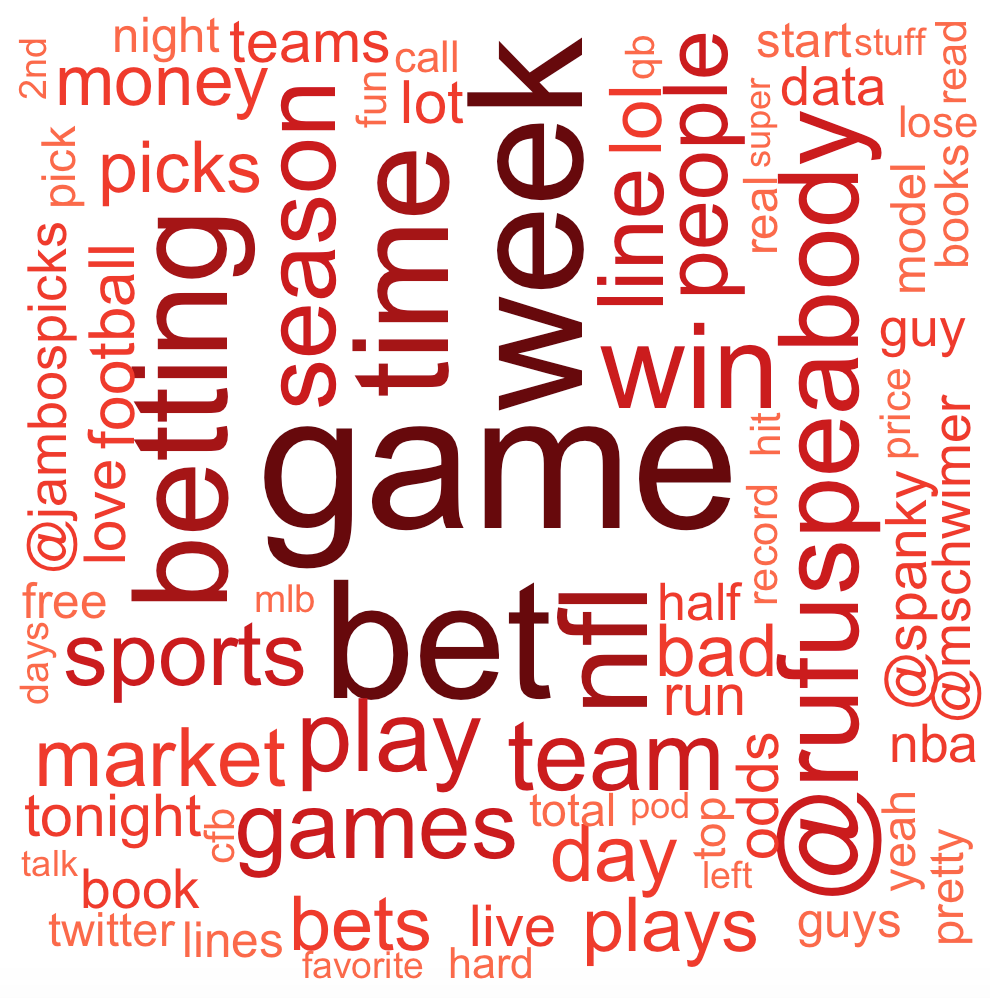
\includegraphics[width=3.4in]{figures/Top_Words.png}
	\caption[]{Word cloud of the top words used in the gambling twitter dataset} 
	\label{Top Words} 
\end{figure}


Figure \ref{word_dist} shows the distribution of the number of words used in each tweet. There are substantially more shorter tweets than longer tweets making it much more difficult for the model to capture the personality of each user. The average number of words in a tweet is just 18.42, with the median number of words at only 14. 

\begin{figure}[!htb] \centering
	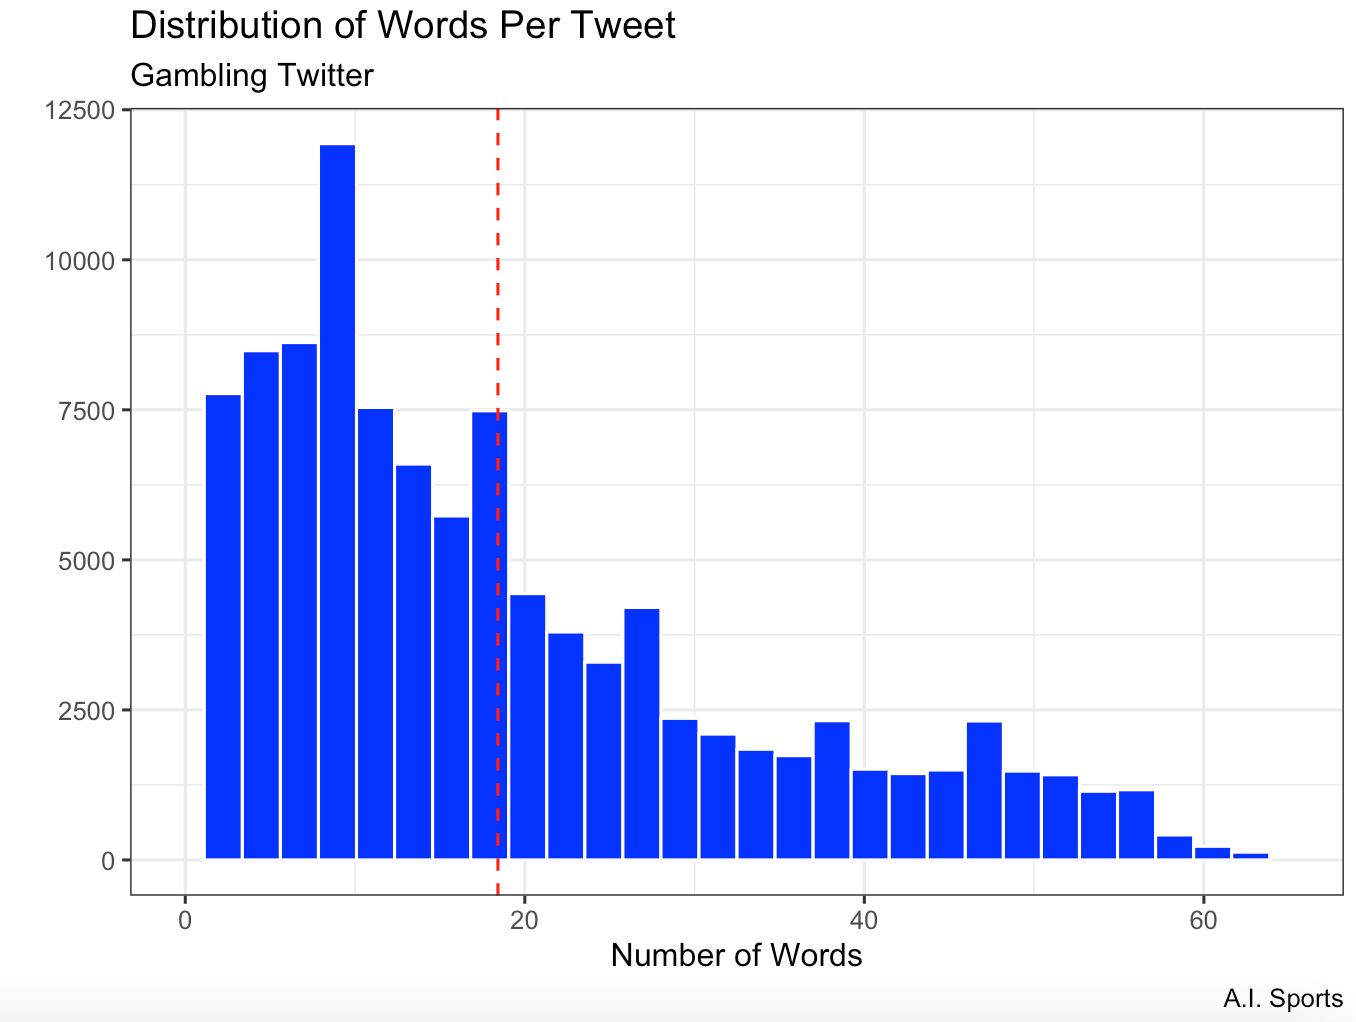
\includegraphics[width=3.4in]{figures/Words_per_Tweet.png}
	\caption[]{Distribution chart of the number of words used per tweet in the dataset} 
	\label{word_dist} 
\end{figure}


The dataset will be split into training, validation, and testing datasets at a 64-16-20 proportion. Using 80\% of the complete dataset for the training and validation process will provide our neural networks enough data to learn differences between each gambling twitter user. These data splits are used to help combat the issues of overfitting and bias. The remaining 20\% proportion of the dataset will be reserved for testing purposes providing a completely unseen sample to judge which of the four models performs best in the real world. 


\subsubsection{Input Data}

Each observation in the dataset represents a single tweet by a gambling twitter user. Each tweet has been transformed by way of tokenization and utilization of a pretrained embedding layer. The word embedding model used for this study is the Word2Vec model created by Thomas Mikolov. The Word2Vec word embedding algorithm creates a vector with a dimension of 300; in other words, each individual word will be represented by a vector of 300 numbers. This embedding model matches with 63\% of the 44,031 unique words in the dataset. The unmatched words will have randomly initialized weights.

The topics in the Google News articles that the Word2Vec embeddings layers were trained on are diverse enough to cover the majority of natural language processing problems. However, sports betting terminology can be fairly unique. While the words used in the tweets may match words in the word2vec model, there may be slightly different meanings attached. Between the GloVe wiki model, GloVe Twitter model, and the Word2Vec model, the Word2Vec model produced the highest lift in the predictive power in the four models trained for this study. 

While Twitter limits each tweet to 256 total characters, the total number of words vary dramatically between each tweet. The maximum sequence of words fed into the algorithms will be set at 50. Tweets with over 50 words will be truncated and tweets with less than 50 words will be padded with zeros to provide consistent sequence lengths for the models to work with.



\subsubsection{Target Data}

This particular modeling scenario is a classification problem. The target variable is a categorical variable with 42 different classes, one for each gambling twitter user in the dataset. These models may struggle determining exactly which user tweeted which tweet because of the small sample size and the strong similarities between users in the gambling twitter space. But there is an opportunity from the modeling to see which users have the most similarities by analyzing the distribution of misclassified predictions among the users.


\section{Computational Experiment and Results}

The entire Python code for this analysis can be reproduced using \href{https://colab.research.google.com/drive/1az7JymjPVX82GoGPvbGTjY9OV8FKhP0A}{Google Notebook Link Collaboratory Notebook} at this url:\\

\href{https://colab.research.google.com/drive/1az7JymjPVX82GoGPvbGTjY9OV8FKhP0A}{https://colab.research.google.com/drive/1az7JymjPVX82GoGPvbGTjY9OV8FKhP0A} \\


The Python Notebook walks through each step from importing the data, loading and mapping embedding layers, building each deep neural network, and evaluating the results.



\subsection{Dense Neural Network (DNN)}

The first deep neural network in the experiment will be a dense, or fully, connected neural network (DNN). This model begins with the Word2Vec embedding layer followed by a layer to reshape, or flatten, the input data. Each tweet is fed into the model as two-dimensional matrix with a shape of 50x300, 50 words in each sequence and 300 numbers to represent each word. The flattening layer reshapes each input into a single row vector with 15,000 values.

The flat data is then connected to a dense layer with 64 nodes. There is a 20\% dropout layer between this dense layer and the final dense output layer. Figure \ref{DNN Summary} shows the structure of this model along with the number of total parameters in each layer.


\begin{figure}[!htb] \centering
	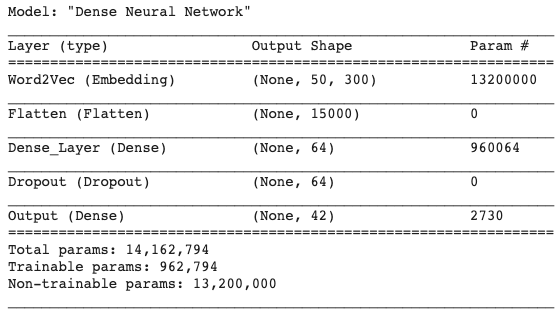
\includegraphics[width=3.4in]{figures/DNN_Model.png}
	\caption[]{Dense Neural Network Model Summary } 
	\label{DNN Summary} 
\end{figure}


\begin{figure}[!htb] \centering
	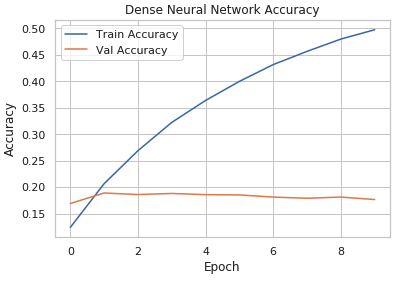
\includegraphics[width=3.4in]{figures/DNN_Accuracy.png}
	\caption[]{Dense Neural Network Training Results} 
	\label{DNN Results} 
\end{figure}


Figure \ref{DNN Results} shows the accuracy of the DNN model as it was trained over the 10 epochs. This model reached a maximum training accuracy of 49.74\% on the training dataset but only reached 18.88\% accuracy on the validation dataset. The problem here is that the peak accuracy on the validation dataset was in the second epoch. From there the validation loss metric reversed course over the duration of the training process. This is a sign that this type of model is not suited for this complex natural language processing problem with the accompanying dataset. The training process was relatively short taking up only 2 minutes and 29 seconds for the 10 epochs.  


\subsection{1D Convolutional Neural Network (CNN)}

The second model, a one-dimensional convolutional neural network (CNN), begins the same way as the DNN model utilizing the Word2Vec embedding layer. The embedding layer is then fed directly into a convolutional layer with 250 filters and a window size of three words. There is a 30\% dropout layer followed by another convolutional layer. Another dropout layer of 30\% occurs between the convolutional layer and the max pooling layer. Once the features have been pooled together, they are densely connected to the output layer. Figure \ref{CNN Summary} provides a detailed summary of this model.


\begin{figure}[!htb] \centering
	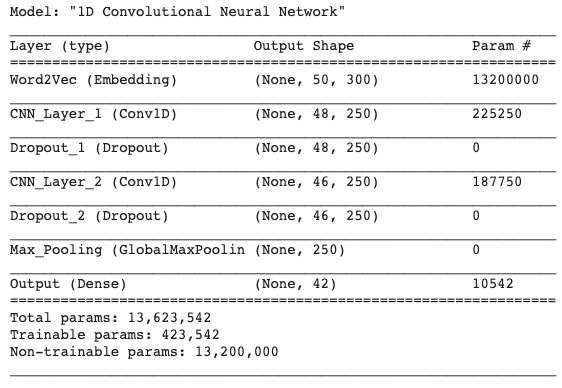
\includegraphics[width=3.4in]{figures/CNN_Model.png}
	\caption[]{One-Dimensional Convolutional Neural Network Model Summary} 
	\label{CNN Summary} 
\end{figure}


\begin{figure}[!htb] \centering
	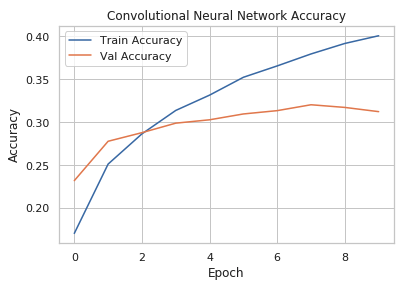
\includegraphics[width=3.4in]{figures/CNN_Accuracy.png}
	\caption[]{One-Dimensional Convolutional Neural Network Training Results} 
	\label{CNN Results} 
\end{figure}


Figure \ref{CNN Results} shows the accuracy of this model as it was trained over the 10 epochs. The CNN model achieved 40.08\% accuracy on the training dataset and peaked at 32.04\% accuracy on the validation dataset. The maximum accuracy on the validation dataset took place during the 8th epoch. The final two epochs show signs of overfitting on the training dataset as the gap between training and validation accuracy grew. The one-dimensional convolutional neural network took 6 minutes and 57 seconds to complete the 10 epochs. That is a 180\% increase in time over the DNN model but with much better accuracy. 


\subsection{Recurrent Neural Network (RNN)}


The LSTM recurrent neural network (RNN) model flows from the embedding layer into back-to-back LSTM recurrent layers. Each one of the LSTM layers has a 20\% dropout built into them. These layers return full sequences which require a flattening layer before it reaches the dense output layer. Figure \ref{RNN Summary} provides a detailed summary of this model with the number of parameters in each layer and the shape of the data at each layer.


\begin{figure}[!h] 
    \centering
	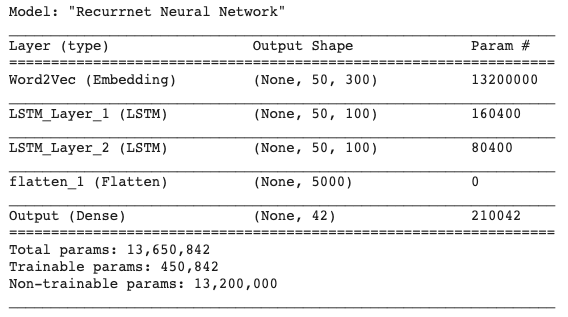
\includegraphics[width=3.4in]{figures/RNN_Model.png}
	\caption[]{Recurrent Neural Network Model Summary} 
	\label{RNN Summary} 
\end{figure}


\begin{figure}[!htb] \centering
	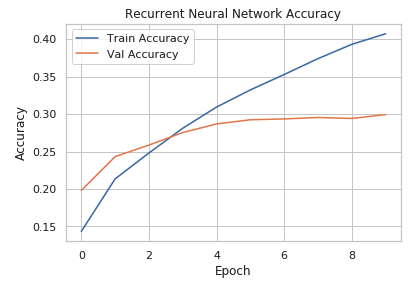
\includegraphics[width=3.4in]{figures/RNN_Accuracy.png}
	\caption[]{Recurrent Neural Network Training Results} 
	\label{RNN Results} 
\end{figure}


Figure \ref{RNN Results} plots the accuracy across the 10 epochs. The RNN model accomplished 40.72\% accuracy on the training dataset and peaked at 29.93\% accuracy on the validation dataset. This model appears to have potential of achieving even better results if the training time was extended. The recurrent neural network took 52 minutes and 45 seconds to train, roughly 7½ times more than the CNN model.



\subsection{Bidirectional Recurrent Neural Network (Bi-RNN)}


The bidirectional recurrent neural network (Bi-RNN) has the exact same form as the previous RNN model except for one critical difference. Each of the LSTM layers is bidirectional processing the data forward and backwards. This doubles the number of trainable parameters. Figure \ref{BiRNN Summary} provides a summary of the model with a breakdown of the total number of parameters and layers.


\begin{figure}[!htb] \centering
	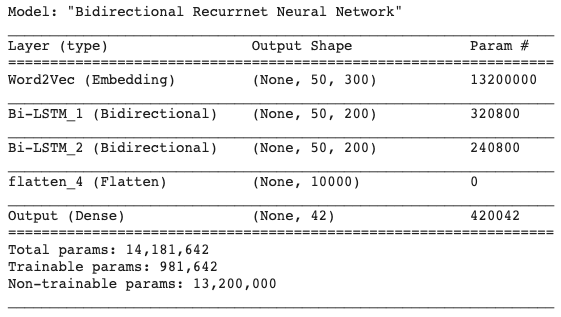
\includegraphics[width=3.4in]{figures/Bi-RNN_Model.png}
	\caption[]{Bidirectional Recurrent Neural Network Model Summary} 
	\label{BiRNN Summary} 
\end{figure}


\begin{figure}[!htb] \centering
	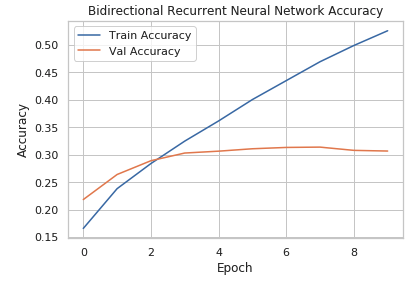
\includegraphics[width=3.4in]{figures/Bi-RNN_Accuracy.png}
	\caption[]{Bidirectional Recurrent Neural Network Training Results} 
	\label{BiRNN Results} 
\end{figure}


Figure \ref{BiRNN Results} plots the accuracy of the Bi-RNN model as it was trained over the 10 epochs. The model was able to learn the training dataset extremely well with a maximum accuracy of 52.6\% accuracy. However, the validation dataset accuracy peaked after 8 epochs at 31.39\%. The Bi-RNN took the longest amount of time to train, clocking in at 1 hour 24 minutes and 1 second, which is an increase of 59\% from the RNN model. 


\section{Model Evaluation}


\begin{table}[!htb] 
  \centering 
  \begin{tabular}{@{\small}llll@{}} 
    \toprule % utilise booktabs
    & {\footnotesize Training Time} &  {\footnotesize Validation Accuracy} & {\footnotesize Test Accuracy} \\ \midrule
    DNN & 2:29 & 18.88\% & 17.38\% \\
    CNN & 6:57 & 32.04\% & 31.50\% \\
    RNN & 52:45 & 29.93\% & 29.43\% \\
    Bi-RNN & 1:24:01 & 31.39\% & 30.35\% \\ 
    \bottomrule
\end{tabular} \caption{Side by Side comparison of the four deep neural networks} \label{table_eval}
\end{table}


Figures \ref{Train Accuracy} and \ref{Val Accuracy} compare each of the models training and validation accuracy respectively. Both the DNN and Bi-RNN were able to learn the training dataset very well as is shown in both their loss and accuracy curves but the DNN model was a clear outlier in Figure \ref{Val Accuracy} and \ref{Val Loss} being unable to generalize to the validation dataset. 

Table 1 compares each model’s training time, validation and test accuracy. The CNN model was the clear winner for this particular natural language processing problem. The training time is significantly shorter requiring much lower computational expense. The RNN and Bi-RNN have very similar results. The Bi-RNN was able to pick up slightly more signal when dissecting the tweets in reverse but the extra time to train might not be worth it depending on the situation. The DNN model failed to differentiate the gambling twitter users.


\begin{figure}[!htb] \centering
	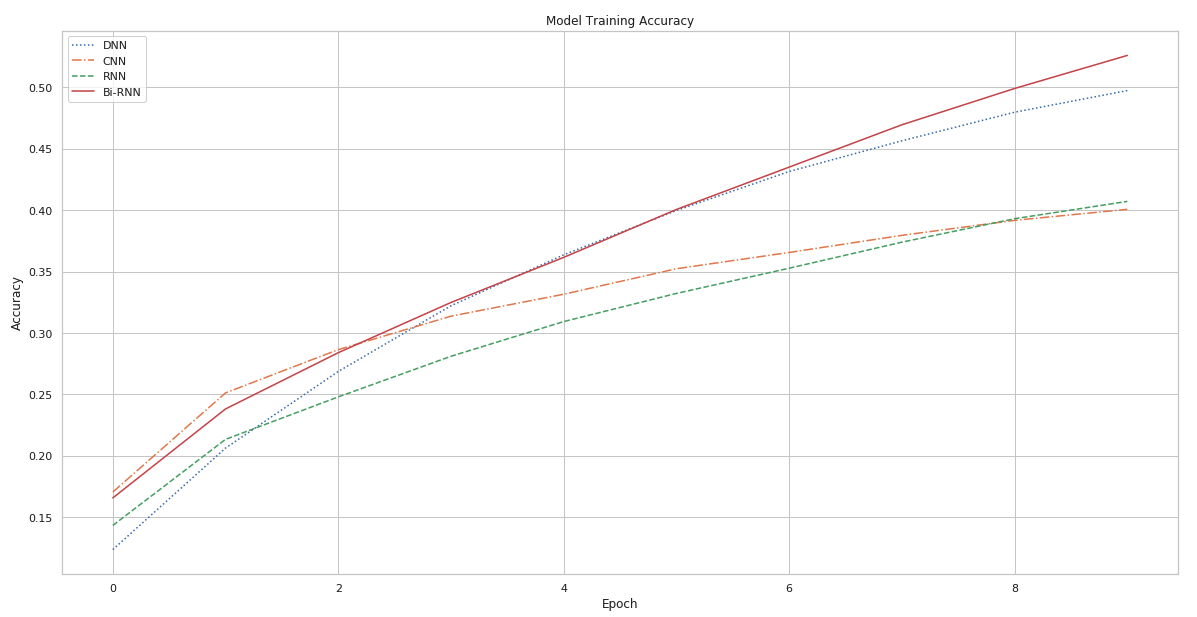
\includegraphics[width=3.4in]{figures/All_Train_Acc.png}
	\caption[]{Training Accuracy Comparison between the 4 models} 
	\label{Train Accuracy} 
\end{figure}


\begin{figure}[!htb] \centering
	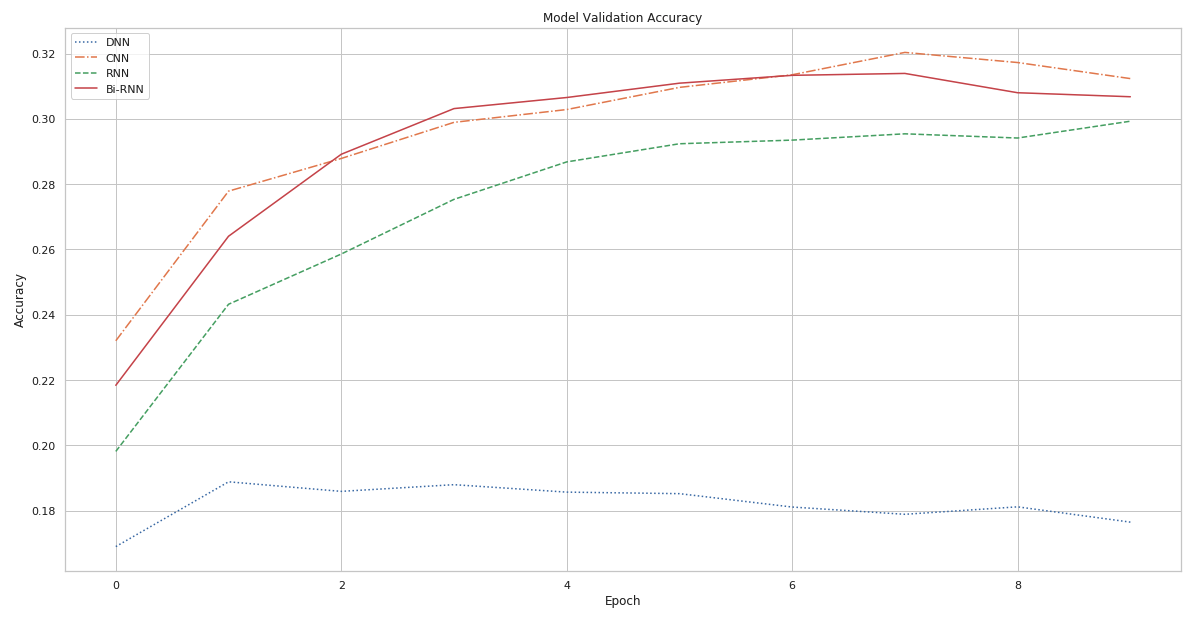
\includegraphics[width=3.4in]{figures/All_Val_Acc.png}
	\caption[]{Validation Accuracy Comparison between the 4 models} 
	\label{Val Accuracy} 
\end{figure}

\begin{figure}[!htb] \centering
	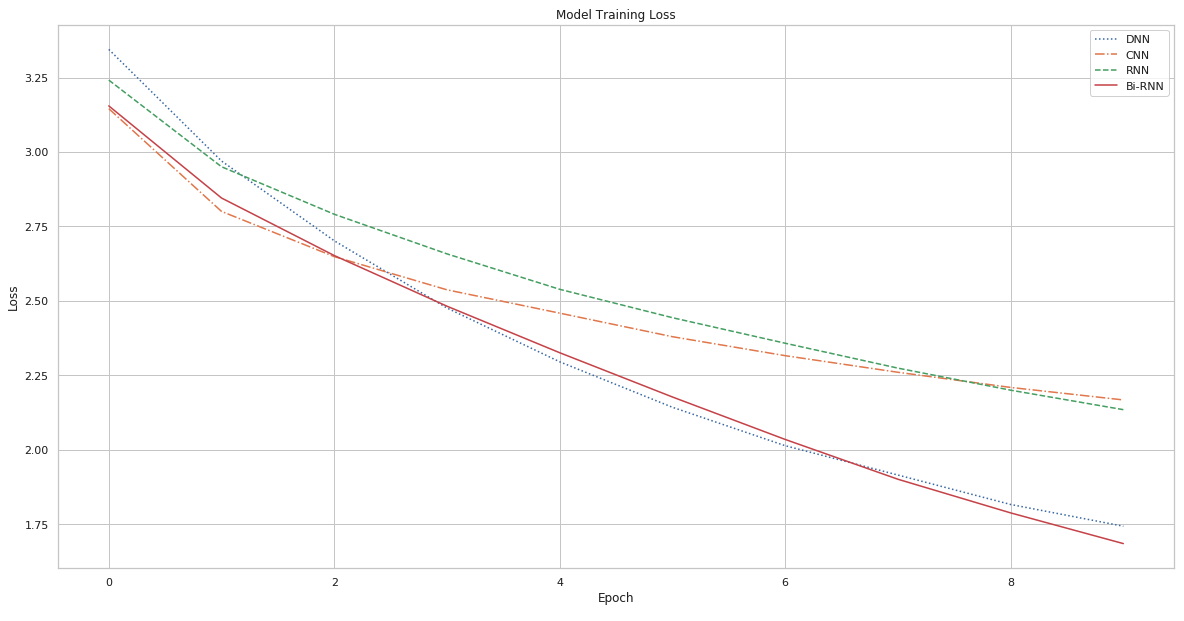
\includegraphics[width=3.4in]{figures/All_Train_Loss.png}
	\caption[]{Training Loss/Cost Comparison between the 4 models} 
	\label{Train Loss} 
\end{figure}

\begin{figure}[!htb] \centering
	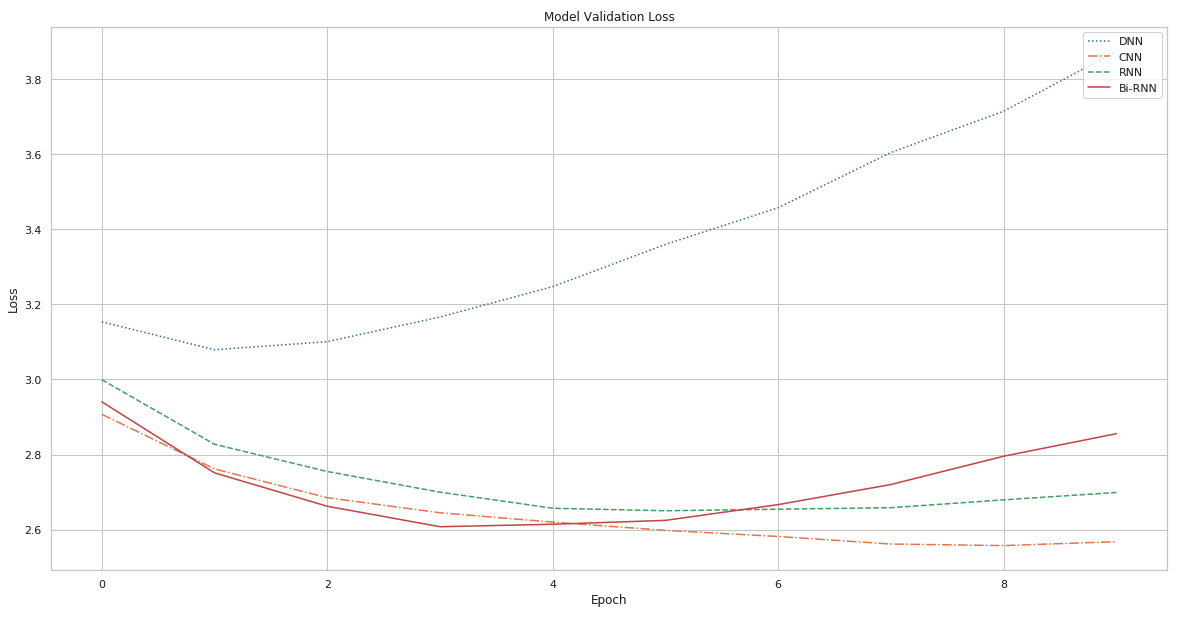
\includegraphics[width=3.4in]{figures/All_Val_Loss.png}
	\caption[]{Validation Loss/Cost Comparison between the 4 models} 
	\label{Val Loss} 
\end{figure}





\section{Discussion and Conclusions}


\begin{figure}[!htb] \centering
	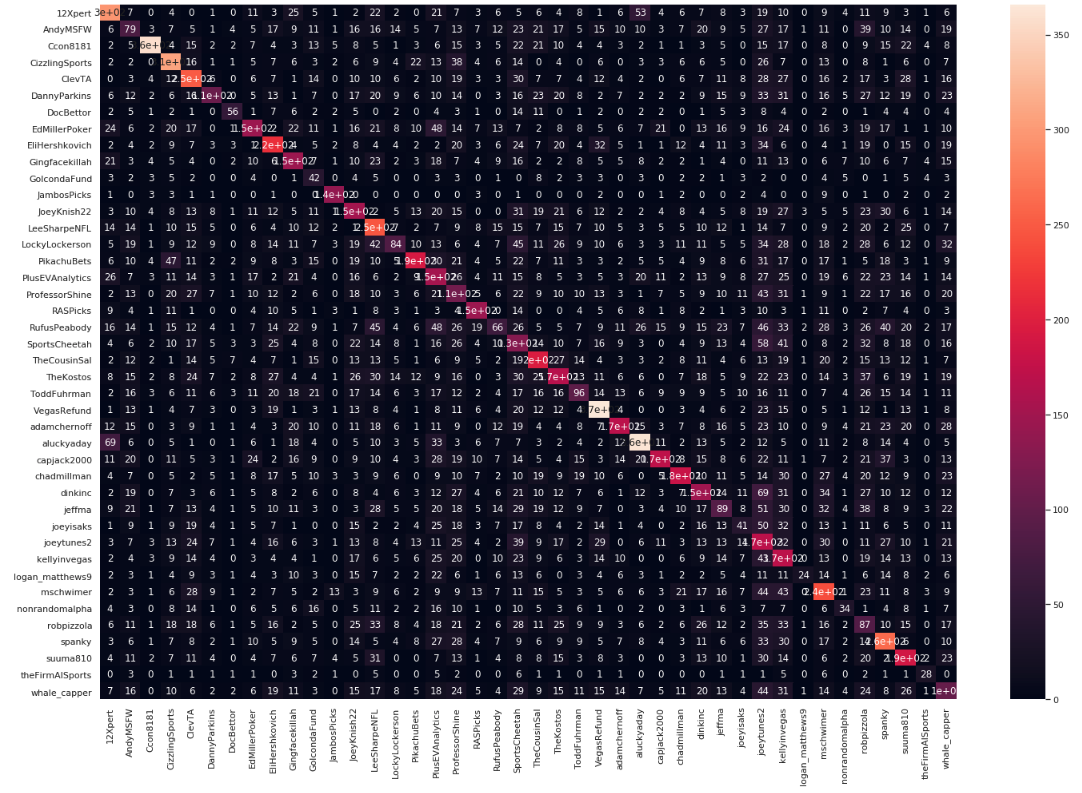
\includegraphics[width=3.4in]{figures/CNN_Confusion_Matrix.png}
	\caption[]{CNN Confusion Matrix Heatmap} 
	\label{Confuse} 
\end{figure}




Figure \ref{Confuse} is a confusion matrix for the winning model, the one-dimensional convolutional neural network. This provides a view of which predictions were correct for each class (A perfect model would only have values in a diagonal through the visual). The top gambling twitter users that the CNN was classify correctly were 1. JambosPicks (78.21\% correct), 2. Vegas Refund (58.75\% correct), 3. Chris Conley (55.94\% correct), and 4. CizzlingSports (54.04\% correct). JambosPicks tweets are very distinct only giving out picks and using their Jambos hashtag with very few miscellaneous tweets. Vegas Refund and Chris Conley are both users who keep the majority of their tweets focused on giving out specific games to bet. Cizzling Sports spends all of his time exposing and criticizing frauds and touts using harsh and strong language.

The CNN model struggled to classify tweets for a handful of users. 1. Rufus Peabody (9.27\% correct), 2. Logan Matthews (9.6\% correct), and 3. JoeyIsaks (10.68\% correct). Rufus Peabody tweets about anything and everything. He is a thought leader and key voice in the gambling world. This model had an unusally high portion of Rufus’ tweets misclassified as PlusEVanalytics (6.7\%) and Joey Tunes (6.5\%) indicating strong similarity between them. As for Logan Matthews and JoeyIsaks, they both had smaller sample sizes making it difficult for the algorithm to effectively learn their tendencies.

Potential future work to improve the accuracy of these models would include training specific word embeddings on a dedicated sports betting and twitter corpus. This would help capture some of the contextual meaning and unique topics discussed between these twitter users. Increasing the sample size for each gambling twitter user will also improve the results. It is difficult to differentiate 42 people. Fine tuning hyperparameters and layer architecture may provide improved modeling results.

Overall, the goals of this study were accomplished. A trustworthy deep neural network was carefully crafted to successfully identify which gambling twitter users tweeted which tweet. The limitations of the models are known and potential steps to improve the accuracy are laid out. The models were able to provide greater insights into which users have a similar voice in this space and which users are more distinct. Recurrent neural networks and one-dimensional convolutional neural networks are extremely powerful and useful models for natural language processing tasks.


\bibliography{bibliographie.bib}

\bibliographystyle{newapa}

\end{document}